\documentclass[11pt,a4paper]{article}
\usepackage[T1]{fontenc}
\usepackage{lmodern}
\usepackage[margin=2.3cm]{geometry}
\usepackage{microtype}
\usepackage{amsmath,amssymb}
\usepackage{graphicx}
\usepackage{booktabs,tabularx}
\usepackage{enumitem}
\usepackage[dvipsnames]{xcolor}
\usepackage{listings}
\usepackage{caption}
\usepackage{fancyhdr}
\usepackage{titlesec}
\usepackage[colorlinks=true,linkcolor=MidnightBlue,urlcolor=MidnightBlue,citecolor=MidnightBlue]{hyperref}

\definecolor{aether}{HTML}{0A9BB8}
\definecolor{violet}{HTML}{6B5CE0}
\definecolor{codebg}{HTML}{F3F7FA}
\titleformat{\section}{\Large\bfseries\color{aether!70!black}}{\thesection}{0.8em}{}
\titleformat{\subsection}{\large\bfseries}{\thesubsection}{0.8em}{}
\lstset{basicstyle=\ttfamily\small,backgroundcolor=\color{codebg},frame=single,rulecolor=\color{codebg},
        breaklines=true,columns=fullflexible,keepspaces=true,xleftmargin=4pt,xrightmargin=4pt}
\setlist{itemsep=2pt,topsep=4pt}
\pagestyle{fancy}\fancyhf{}
\fancyhead[L]{\small\textsc{AETHER} technical report}\fancyhead[R]{\small\thepage}
\renewcommand{\headrulewidth}{0.3pt}
\usepackage[htt]{hyphenat}
\newcommand{\code}[1]{\texttt{#1}}

\title{\vspace{-1.2cm}\textbf{\color{aether!80!black}AETHER}\\[4pt]
\large Adaptive Engine for Thought, Heuristics, Evolution \& Reasoning\\[2pt]
\normalsize A fully local, neuro-symbolic personal assistant for Windows~11}
\author{Aryan Khanna}
\date{Technical report on the state at Phase 13 \quad·\quad 25 November 2026}

\begin{document}
\maketitle
\thispagestyle{empty}

\begin{abstract}
\noindent AETHER is a personal assistant in the spirit of a ``Jarvis'' that runs entirely on one laptop: an HP Victus~15 with a 4\,GB RTX~3050 GPU, a Ryzen~5 5600H and 16\,GB of RAM. It uses no cloud APIs and no model server; a quantised 7B language model runs in-process through \code{llama.cpp}. The central design idea is that the language model is \emph{not} the whole brain. The model interprets requests and writes answers, while deterministic code validates its output, routes retrieval, reasons over a temporal knowledge graph with forward-chaining rules, solves constraint problems exactly, gates every action through a policy engine and checks the final answer against known facts. Around this core sit layered encrypted memory, cited research over local documents and the web, multi-agent background goals, computer control, personalisation, a wellness companion, voice and vision, six metaheuristic optimisers, metacognition and a proactive engine. The latest phase makes the system inspectable: every turn is traced, the user can ask counterfactual ``what if'' questions of the knowledge graph, replay how beliefs changed over time, watch agents execute a goal graph and talk to it through a full-screen voice interface. This report describes the architecture, the algorithms, the security model, how the system was tested and what remains.
\end{abstract}

\tableofcontents
\newpage

%=====================================================================
\section{Goals and constraints}

AETHER was specified as a maximum-ambition personal assistant with four hard constraints:

\begin{enumerate}
  \item \textbf{Fully local.} No hosted APIs and no Ollama. The language model, embeddings, speech-to-text, text-to-speech and vision all run in-process on the user's machine. The only network use is optional web research, which can be switched off.
  \item \textbf{Windows 11 on modest hardware.} The defaults are tuned for 4\,GB of VRAM: Qwen2.5-7B-Instruct at Q4\_K\_M with 20 of 28 layers on the GPU and the rest on six CPU threads, flash attention on, a 6\,144-token context and a 256-token batch. Embeddings, speech and vision run on the CPU so the GPU stays free for the main model.
  \item \textbf{Verifiable autonomy.} Every action passes a policy engine, risky actions require approval, everything is audited and file changes can be undone.
  \item \textbf{Inspectable learning.} Every memory, fact, preference and observation can be seen, corrected and deleted, and from Phase~13 every reasoning step can be inspected after the fact.
\end{enumerate}

\section{Architecture}

\begin{figure}[h]
  \centering
  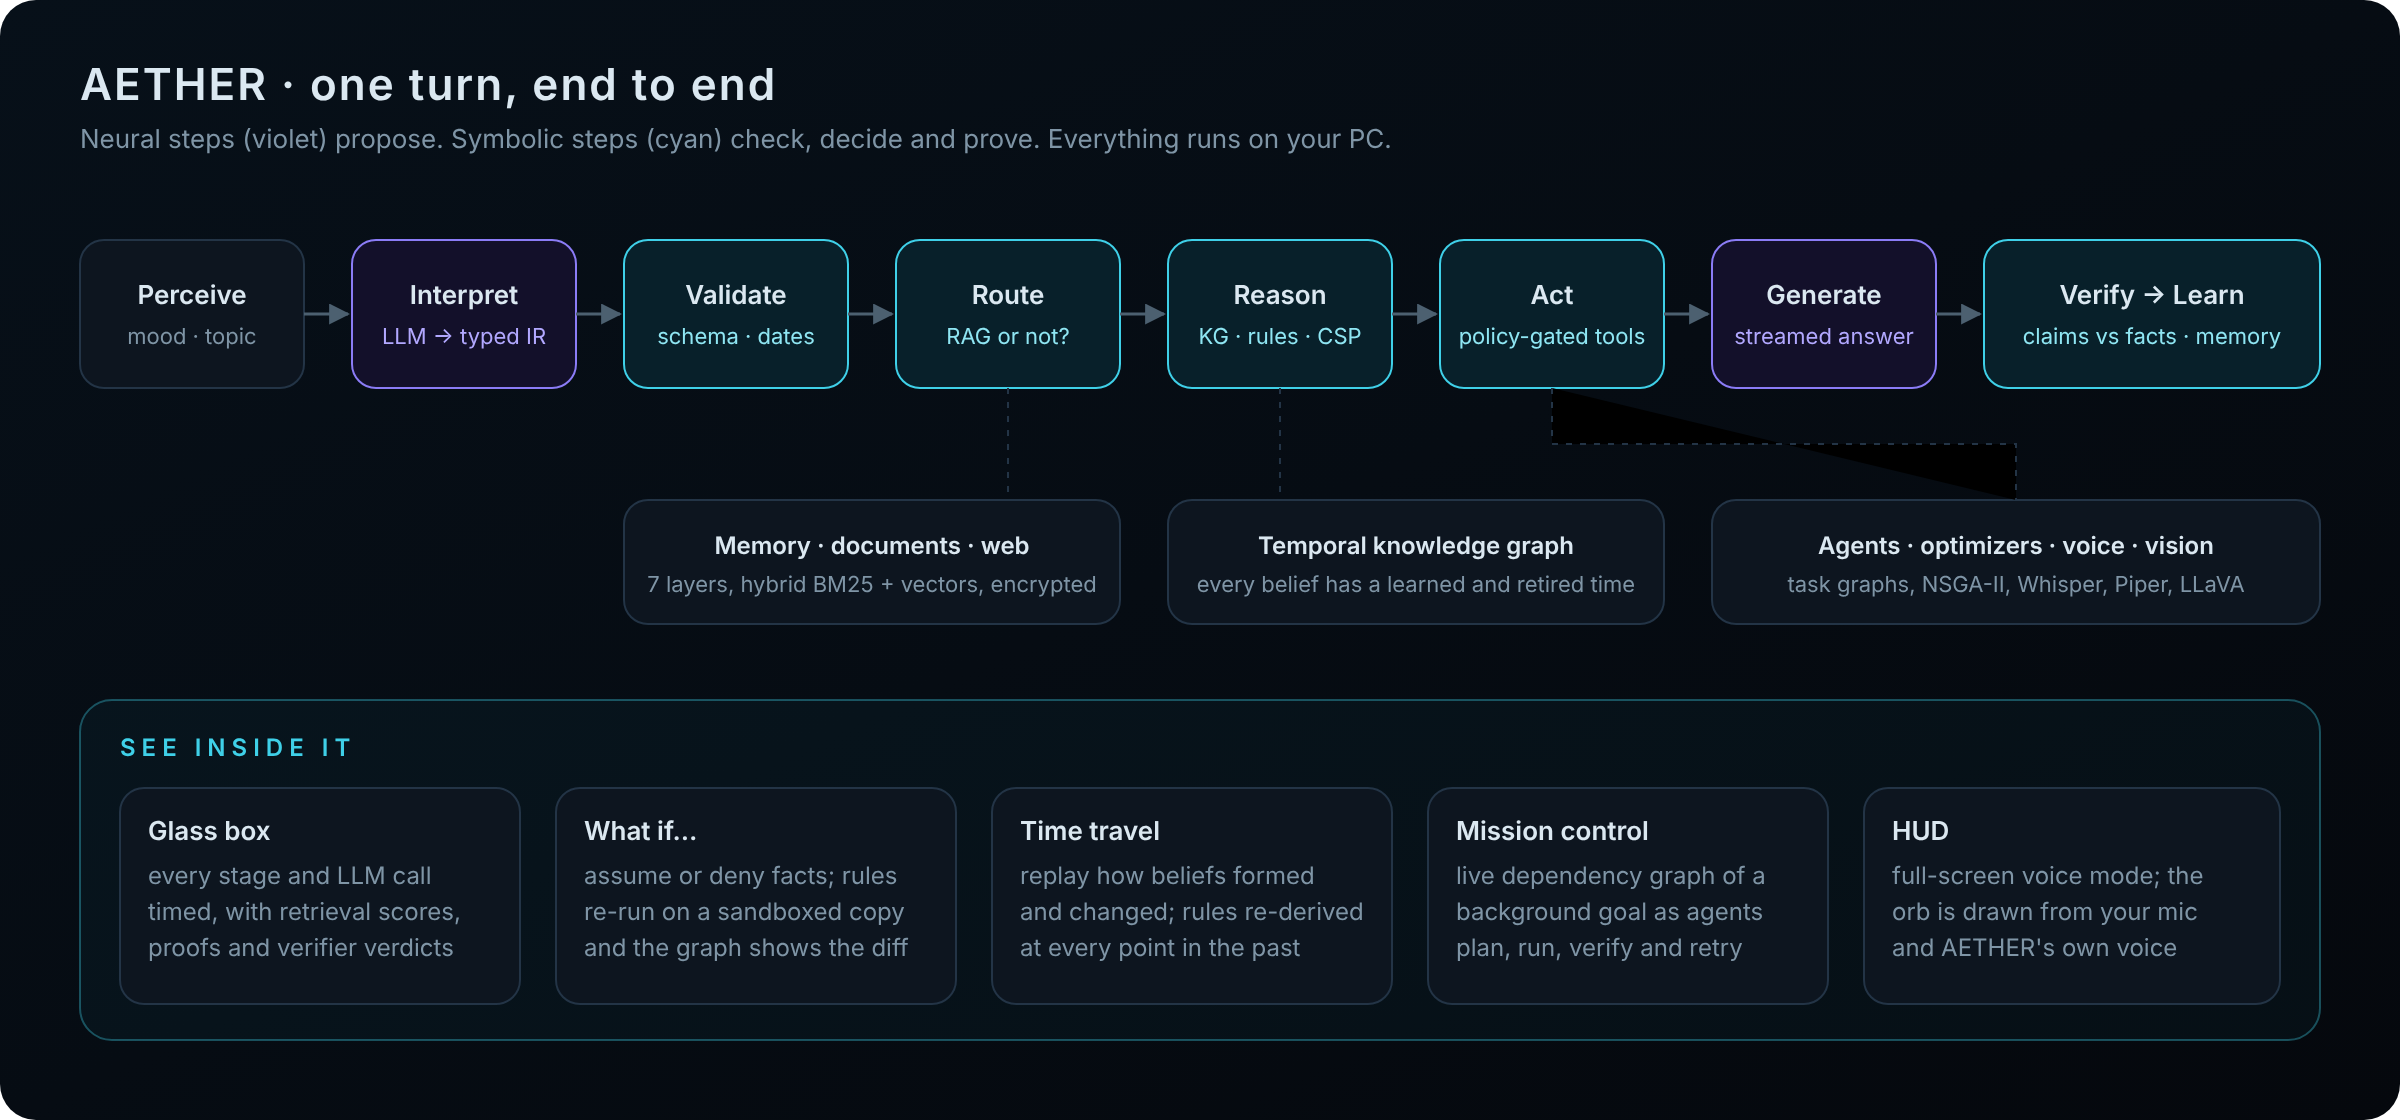
\includegraphics[width=\linewidth]{architecture.png}
  \caption{One turn through AETHER. Neural steps (violet) propose; symbolic steps (cyan) check, decide and prove. The lower band is the Phase~13 inspection layer.}
\end{figure}

\subsection{The turn pipeline}

Each user message passes through a fixed sequence of stages, implemented in \code{aether/\allowbreak cognition/\allowbreak orchestrator.py}. Each stage emits live events (\code{stage}, \code{tool}, \code{token}, \code{replace}, \code{done}) that the web app streams to the user.

\begin{center}
\begin{tabularx}{\linewidth}{@{}l l X@{}}
\toprule
Stage & Kind & What happens \\
\midrule
Perceive & code & Wellness check (crisis, stress, neutral), topic tracking, preference feedback detection \\
Interpret & LLM & Message $\rightarrow$ typed \code{IntentIR}, decoded under a JSON-schema grammar so it always parses \\
Validate & code & Resolve relative dates, drop unknown tools, ambiguity gate \\
Learn & code & Stated facts go into the knowledge graph; contradictions are flagged \\
Retrieve & code & Router picks: direct, memory, documents, web, symbolic, tools or optimise \\
Reason & code & Forward-chaining rules to a fixpoint, integrity constraints, proofs \\
Act & LLM + code & The model proposes tool calls; the policy engine decides \\
Generate & LLM & Answer from trusted facts and clearly separated untrusted data, streamed \\
Verify & LLM + code & The model extracts claims; code checks them against the graph and removes invented citations \\
\bottomrule
\end{tabularx}
\end{center}

\subsection{The intermediate representation}
The interpreter produces an \code{IntentIR}: an intent label, a one-line objective, entities, constraints, time expressions, \code{facts\_stated} as subject--predicate--object triples, retrieval needs, required tool calls, an emotional tone, an ambiguity note and a confidence. Because the model decodes under a grammar derived from the Pydantic schema, the output is always valid JSON; it is still validated and retried once with the error fed back. Downstream code never reads free text from the model when a typed field exists, which makes the rest of the pipeline deterministic and testable.

%=====================================================================
\section{The neuro-symbolic core}

\subsection{Temporal knowledge graph}
Facts are triples $(s,p,o)$ stored in SQLite with a source (\code{user\_stated}, \code{document}, \code{inferred}, \ldots), a confidence, a creation time and an optional retirement time $t_{\mathrm{valid\_to}}$. Entity names are normalised (lower case, spaces to underscores). Predicates are typed: \emph{symmetric} predicates such as \code{sibling\_of} are stored both ways, \emph{inverse} pairs are maintained, and \emph{functional} predicates such as \code{lives\_in} hold a single value, so asserting a new value retires the old one instead of deleting it. The belief state at any time $t$ is therefore
\[
  K(t) = \{(s,p,o) \mid t_{\mathrm{created}} \le t \;\wedge\; (t_{\mathrm{valid\_to}} = \bot \;\vee\; t_{\mathrm{valid\_to}} > t)\},
\]
which powers both contradiction detection and Phase~13's time travel.

\subsection{Rule engine}
Rules are Datalog-style Horn clauses with variables, for example
\begin{lstlisting}
parent_of(?g, ?p) & parent_of(?p, ?c) -> grandparent_of(?g, ?c)
works_at(?x, ?org) & located_in(?org, ?city) -> works_in(?x, ?city)
depends_on(?a, ?a) -> !circular_dependency(?a, ?a)
\end{lstlisting}
A head prefixed with \code{!} is an integrity constraint: if the body matches, that is a violation. The engine forward-chains to a fixpoint (bounded at ten rounds) by matching rule bodies against the fact set with backtracking unification. Every derived fact keeps a \emph{proof}: the rule and the supporting facts. The user can ask \emph{why} and receive the proof tree, add rules of their own, and query the graph with conjunctive patterns such as \code{parent\_of(?p, riya) \& lives\_in(?p, ?c)}. Nine rules ship by default, covering family, location, part--whole and dependency transitivity, taxonomies and three integrity constraints.

\subsection{Exact planning}
Scheduling with hard deadlines and dependencies is solved exactly by a small constraint solver (backtracking with forward checking over day assignments) rather than by the language model. When the user wants trade-offs instead of a single feasible answer, the metaheuristics of Section~\ref{sec:opt} take over.

\subsection{Answer verification}
After generation the model extracts the factual claims in its own draft as triples. Code then checks each claim against the graph: supported claims pass, claims that contradict a stated fact trigger a rewrite before the user sees the answer, and citation markers such as \code{[doc 2]} that do not correspond to a retrieved source are removed. Crisis replies bypass the model entirely for their safety content.

%=====================================================================
\section{Memory and retrieval}

\subsection{Layered memory}
Memories live in seven layers: episodic, semantic, procedural, preference, prospective (reminders), observation (patterns AETHER noticed, kept only after the user confirms) and document chunks. Memory text is encrypted at rest. After conversations an extraction step proposes new memories; topics are summarised; reminders fire through the proactive engine; low-confidence inferred memories decay over time.

\subsection{Hybrid search}
Retrieval combines BM25 with dense vectors from a local \code{bge-small-en-v1.5} embedder. For a memory with normalised BM25 score $\ell$, cosine similarity $v$, age $a$ days and confidence $c$,
\[
  \mathrm{score} = \bigl(\alpha v + (1-\alpha)\,\ell\bigr)\cdot\bigl(0.85 + 0.15\cdot 2^{-a/h}\bigr)\cdot\bigl(0.7 + 0.3c\bigr),
\]
with $\alpha = 0.6$ and half-life $h = 180$ days by default. Results under a minimum score are dropped, so a small-talk message retrieves nothing. An optional cross-encoder reranker can reorder the top hits on the CPU.

\subsection{The router: RAG or not}
A router decides per message whether to retrieve at all and from where, using the IR's declared needs, small-talk detection, the presence of personal pronouns, document references, time-sensitive wording and tool requirements. The result is a list of routes and human-readable reasons, both shown in the user interface and in traces.

\subsection{Documents and research}
A folder watcher keeps authorised folders indexed (text, Markdown, PDF and Word). Documents also feed the knowledge graph: the model extracts triples from them, tagged with their source. The research tool combines web search with local documents and writes a cited brief that separates what the user already knew from what is new. Citations that do not match a real source are removed by code.

%=====================================================================
\section{Agents and autonomy}

Multi-step goals become a persistent task graph. An \emph{executive} agent splits the goal into at most a configured number of tasks, each assigned to a specialist (research, reasoning, coding, operator, memory or verification) with explicit success criteria and dependencies. The plan is validated in code: unknown agents and missing dependencies are rejected and cycles are detected. Tasks whose dependencies are complete run in the background; every result is checked by the verification agent against its success criteria; failed tasks retry with the verifier's feedback up to a bound; if the goal still fails, the executive re-plans once. Each tool call inside a goal still passes through the policy engine, and the user can cancel at any time. Phase~13 renders this graph live as ``mission control'' (Figure~\ref{fig:mission}).

%=====================================================================
\section{Computer control and security}\label{sec:security}

\begin{itemize}
  \item \textbf{Policy engine.} Every tool call has a category (\code{fs.read}, \code{fs.write}, \code{shell}, \code{apps}, \code{screen}, \code{ui}, \ldots). The engine allows, asks or denies based on configuration, authorised folder roots and denylists. AETHER starts read-only; writing needs a separate write root and approval each time.
  \item \textbf{Secrets denylist.} Keys, \code{.env} files, SSH and cloud credentials, browser profiles and credential stores are blocked by path pattern regardless of what the model asks.
  \item \textbf{Prompt-injection defence.} Anything read from files, the web or the screen is untrusted. A scanner looks for instructions aimed at the assistant; if found, the turn is \emph{tainted} and every action needs approval with the reason shown. Untrusted blocks are neutralised before reaching the model.
  \item \textbf{Computer control.} Opening allow-listed applications, a sandboxed shell with an allow-list of programs and a timeout, moves and deletes into a trash with an undo journal, OCR screen reading and UI automation. Screen and UI access are off until enabled.
  \item \textbf{Encryption at rest.} Memories, conversation turns, titles and traces are encrypted with Fernet. On Windows the key is wrapped with DPAPI so it only opens under the user's account.
  \item \textbf{Audit and emergency stop.} Every access and change is written to \code{audit.jsonl} and shown in the Activity view. An emergency stop blocks all actions until the user resumes.
\end{itemize}

%=====================================================================
\section{Personalisation and wellness}

\textbf{Preferences} are learned from direct feedback (``stop the long intros'' takes effect immediately), stored with a timeline of changes, and enforced both in the prompt and by code-side filters (for example removing emojis when the user dislikes them). \textbf{Observations} about behaviour are proposed, never silently adopted. The \textbf{wellness companion} detects stress and chooses among listening, planning, relaxation and other modes, asking ``listen or solve?'' when unsure. Crisis messages always receive helpline information (Tele MANAS 14416 in India, 988 in the US, Samaritans 116\,123 in the UK) guaranteed by code. The companion is supportive conversation, not therapy.

%=====================================================================
\section{Voice and vision}
Speech runs on the CPU: \code{faster-whisper} (\code{small.en}, int8) for speech-to-text, Piper for text-to-speech, energy-based voice activity detection and an openWakeWord model (``hey jarvis''). The voice loop moves between idle, listening, thinking and speaking, supports barge-in (about 240\,ms of clear speech interrupts the reply) and keeps listening for eight seconds after a reply so follow-ups need no wake word. Vision uses a small multimodal GGUF (Qwen2.5-VL-3B) loaded on demand on the CPU to describe images and screenshots.

%=====================================================================
\section{Metaheuristics}\label{sec:opt}
AETHER includes six optimisers written from scratch: a genetic algorithm with elitism, simulated annealing, particle swarm optimisation, tabu search, differential evolution and NSGA-II with fast non-dominated sorting and crowding distance. They power the scheduling workspace (assigning tasks with hours and deadlines to days) and, with NSGA-II, Pareto trade-offs such as finishing early versus balancing load. PSO also \emph{tunes AETHER itself}: given an evaluation set of queries with expected memories, it searches the retrieval parameters $(\alpha, \text{min\_score})$ to maximise
\[
  F_1 = \frac{2\,TP}{2\,TP + FP + FN},
\]
where retrieving anything for an ``expect nothing'' query is a false positive and flooding the context with noise counts against the configuration. Proposed changes go through the metacognition approval flow rather than applying silently.

%=====================================================================
\section{Metacognition and proactivity}
Every turn records latency, route, intent label and confidence (never the user's words). Explicit feedback, implicit signals such as ``that's wrong'' and post-task self-reviews of finished goals produce \emph{proposals} for setting changes, restricted to a whitelist of tunable values and applied only when the user approves. The proactive engine delivers due reminders, a morning brief, finished-goal notices and gentle check-ins, subject to quiet hours (23:00--07:30 by default) and a rate limit of three per hour.

%=====================================================================
\section{Performance on a 4\,GB GPU}
\begin{itemize}
  \item \textbf{Partial offload.} 20 of 28 layers on the GPU keeps VRAM under 4\,GB with room for the KV cache; \code{scripts/tune\_gpu.py} measures the best value on the real machine.
  \item \textbf{Prompt KV cache.} The persona, preferences and tool catalogue are identical every turn. A 768\,MB RAM cache of their key--value state skips re-reading them, which is most of the prompt time on a partly offloaded 7B model.
  \item \textbf{Small-talk fast path.} Greetings and thanks skip interpretation and retrieval entirely.
  \item \textbf{Streaming.} Answers stream token by token, so perceived latency is the time to the first token.
  \item \textbf{CPU for everything else.} Embeddings, speech and vision stay off the GPU.
\end{itemize}
A benchmark script checks these against a performance budget on the user's machine.

%=====================================================================
\section{Interfaces}
AETHER has a terminal chat, a voice loop, a Tauri desktop shell and a local web app served by FastAPI on \code{127.0.0.1:8765}. The web app uses plain ES modules with no build step and loads nothing from the internet. It provides streaming chat with a live ``thinking pipeline'' panel, saved and searchable conversations, a Today view, memory and preference management, an interactive knowledge map, the optimisation lab, self-improvement and audit views, settings, a command palette (\code{Ctrl+K}) and dark and light themes.

\begin{figure}[h]
  \centering
  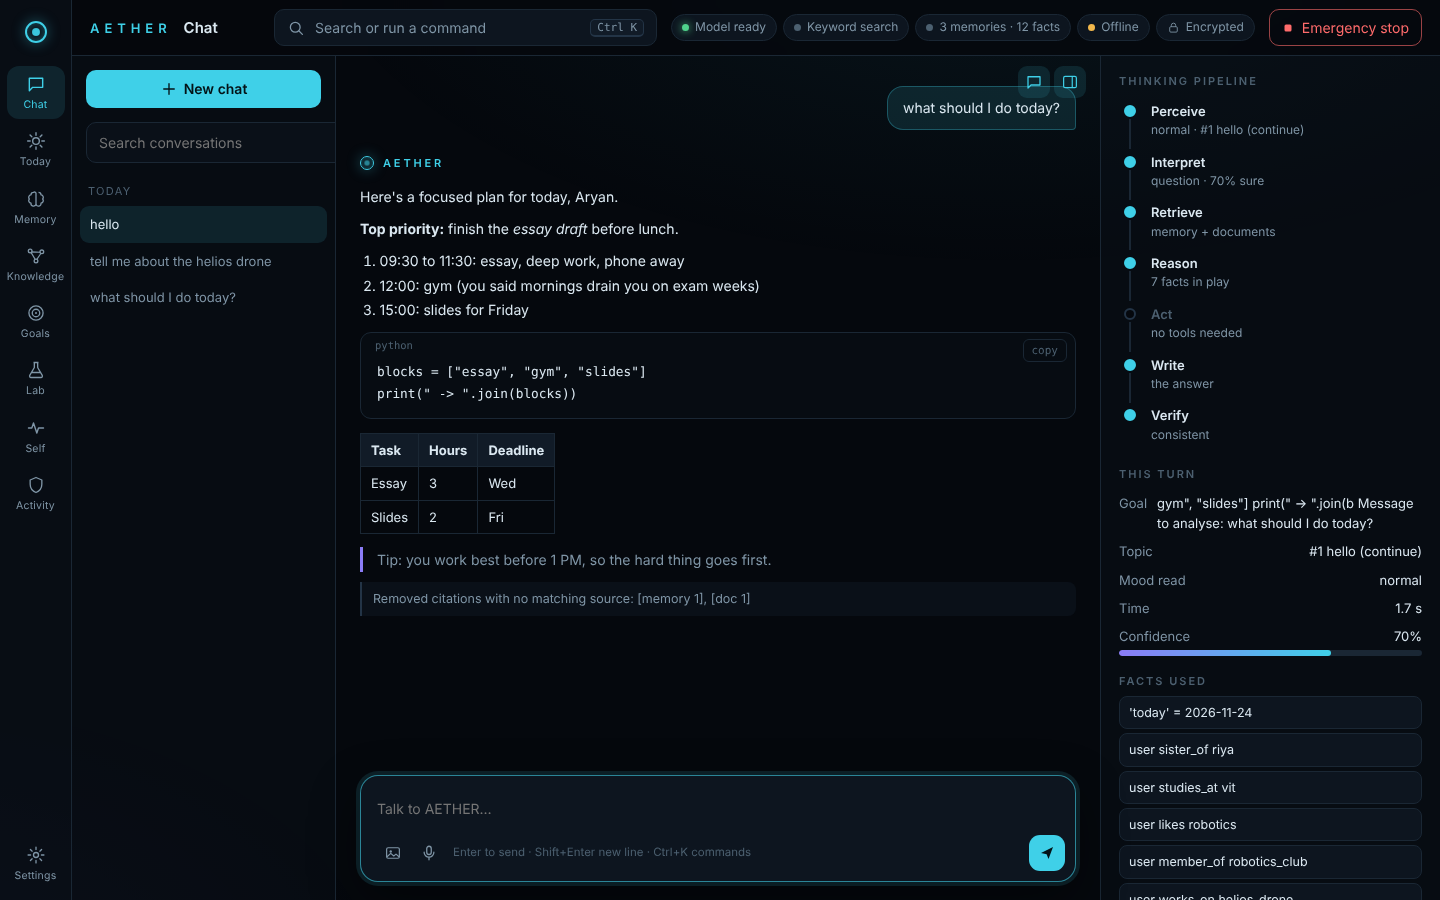
\includegraphics[width=\linewidth]{../screenshots/chat.png}
  \caption{Chat with the live pipeline: each stage, the facts used and the confidence of the answer.}
\end{figure}

%=====================================================================
\section{Phase 13: see inside it}
The latest phase turns AETHER from a black box into a glass box.

\subsection{Glass-box traces}
A recorder wraps the language model for the duration of each turn and times every call (including time to the first streamed token), while stage events are paired into intervals. The resulting trace holds the timeline, retrieved items with their scores, derived facts with their proofs, the verifier's verdicts, notices and the prompt budget split into system, context and history. Traces are encrypted like the rest of the history and can be exported as JSON. An \emph{Inspect} button on each answer opens them as a waterfall.

\begin{figure}[h]
  \centering
  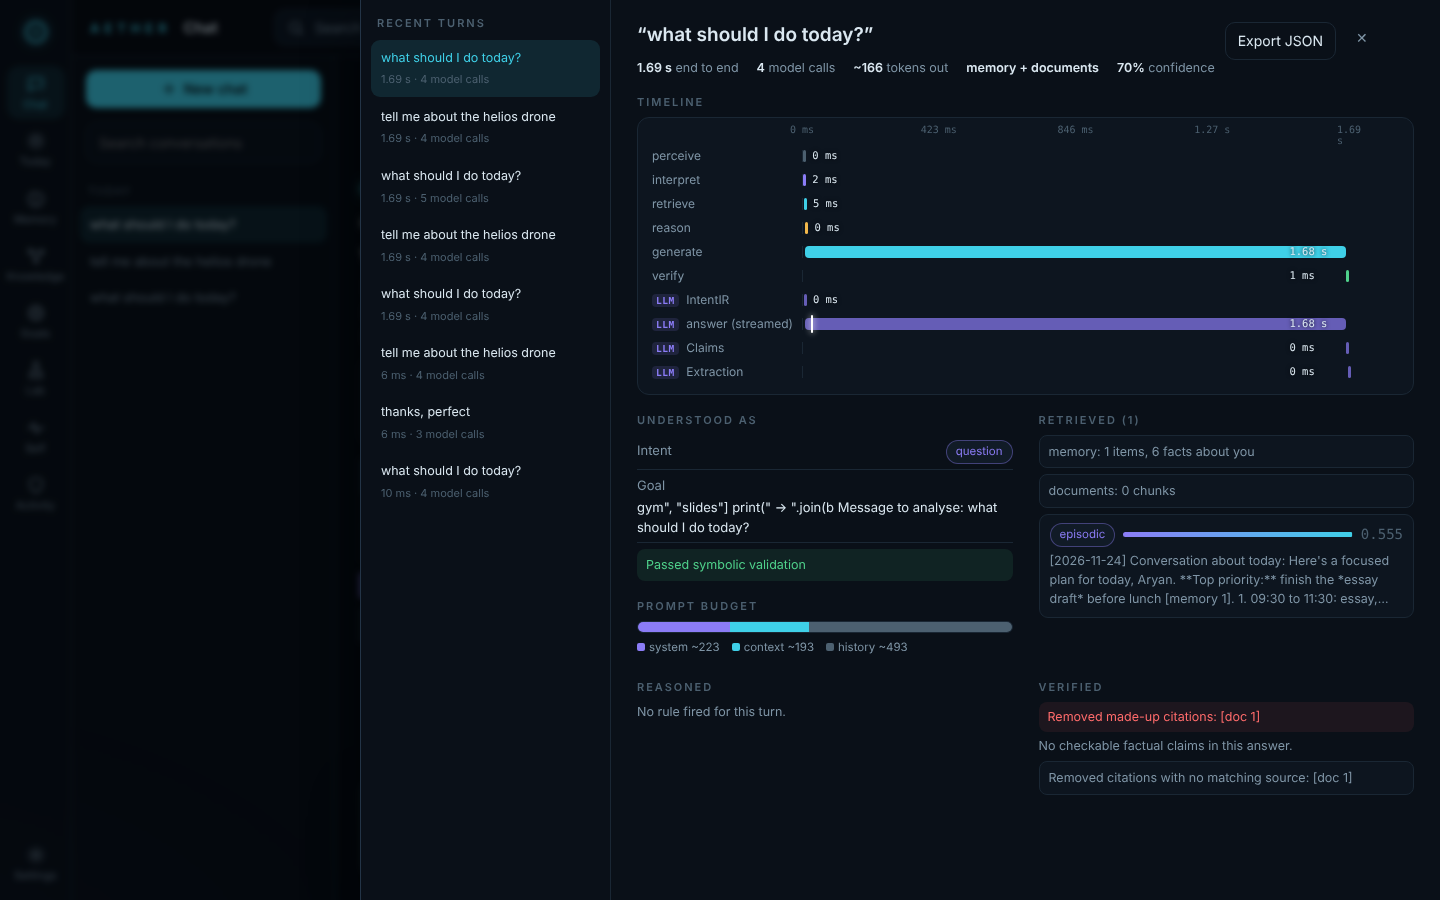
\includegraphics[width=\linewidth]{../screenshots/inspector.png}
  \caption{The inspector: a waterfall of stages and model calls, what was understood, retrieved, derived and verified.}
\end{figure}

\subsection{Counterfactual reasoning}
Given assumptions $A^{+}$ (facts to add) and $A^{-}$ (facts to deny), AETHER copies the live stated facts $S$ into an in-memory graph, applies the change (retiring old values of functional predicates) to obtain $S'$, and computes the rule closure $\mathrm{Cl}(\cdot)$ of both. It reports
\[
  \text{gained} = \mathrm{Cl}(S') \setminus \bigl(\mathrm{Cl}(S) \cup S\bigr),\qquad
  \text{lost} = \mathrm{Cl}(S) \setminus \bigl(\mathrm{Cl}(S') \cup S'\bigr),
\]
together with overridden facts and integrity constraints that newly fail or are resolved. Each gained fact carries its proof. The real graph is never modified. This is available as a chat tool and as a panel that highlights the difference on the knowledge map.

\begin{figure}[h]
  \centering
  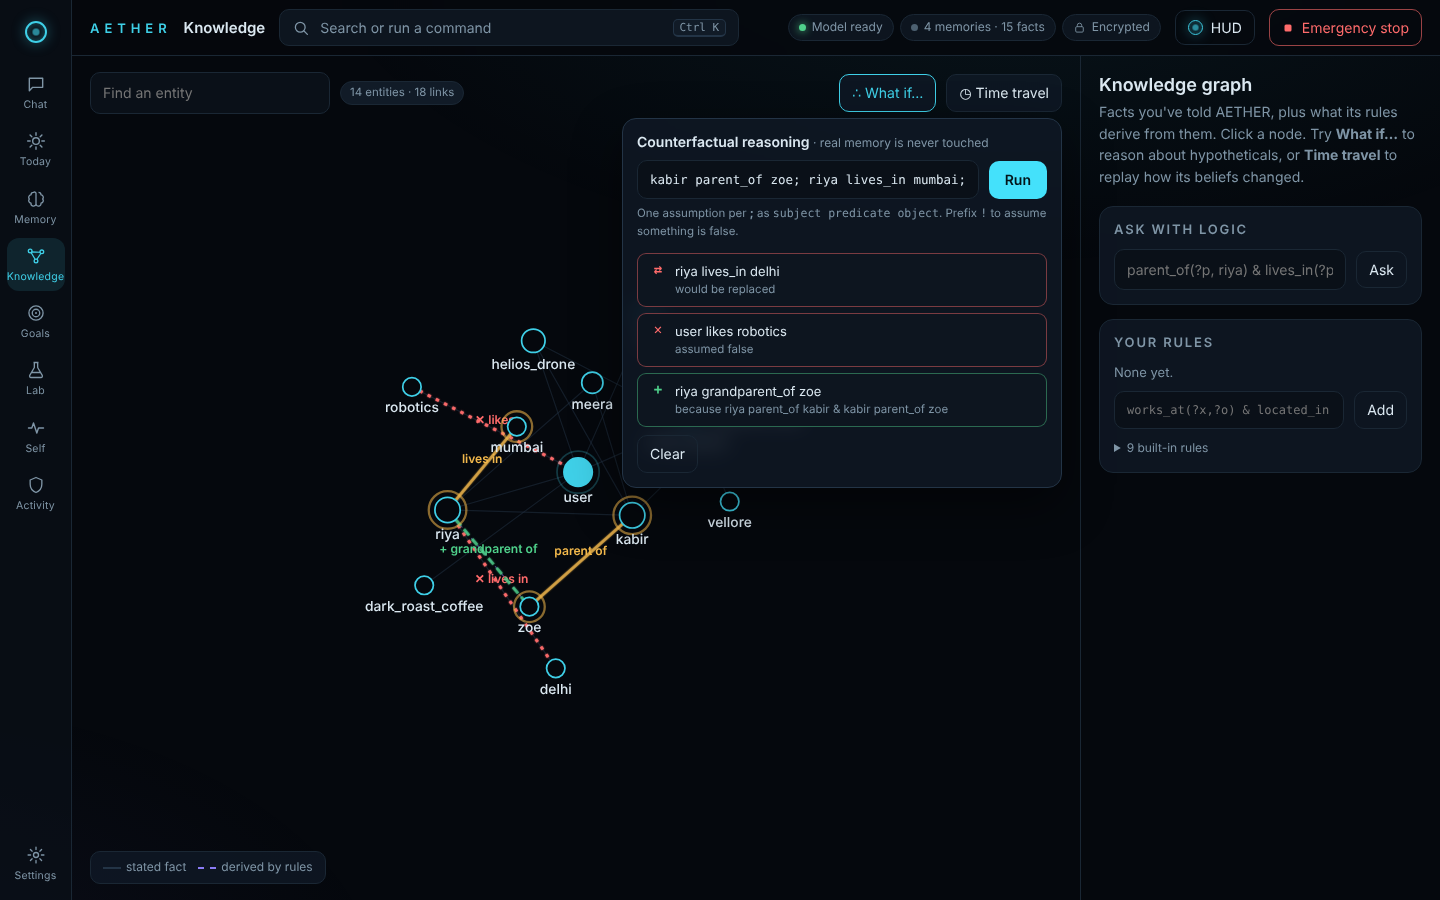
\includegraphics[width=\linewidth]{../screenshots/whatif.png}
  \caption{``What if Kabir had a daughter Zoe, Riya moved to Mumbai, and I no longer liked robotics?'' New conclusions are green, lost ones red, assumptions amber.}
\end{figure}

\subsection{Belief time travel}
Using $K(t)$ from Section~3.1, the knowledge map can be scrubbed or played through every moment at which a belief was learned or retired, with the rules re-derived over each past state. Each entity also has a belief history listing when every fact about it was learned and replaced.

\subsection{Mission control}
Background goals are drawn as a layered dependency graph: tasks are placed by the length of their longest dependency chain, coloured by status, and edges into running tasks animate. The view refreshes every 1.5 seconds while the goal runs.

\begin{figure}[h]
  \centering
  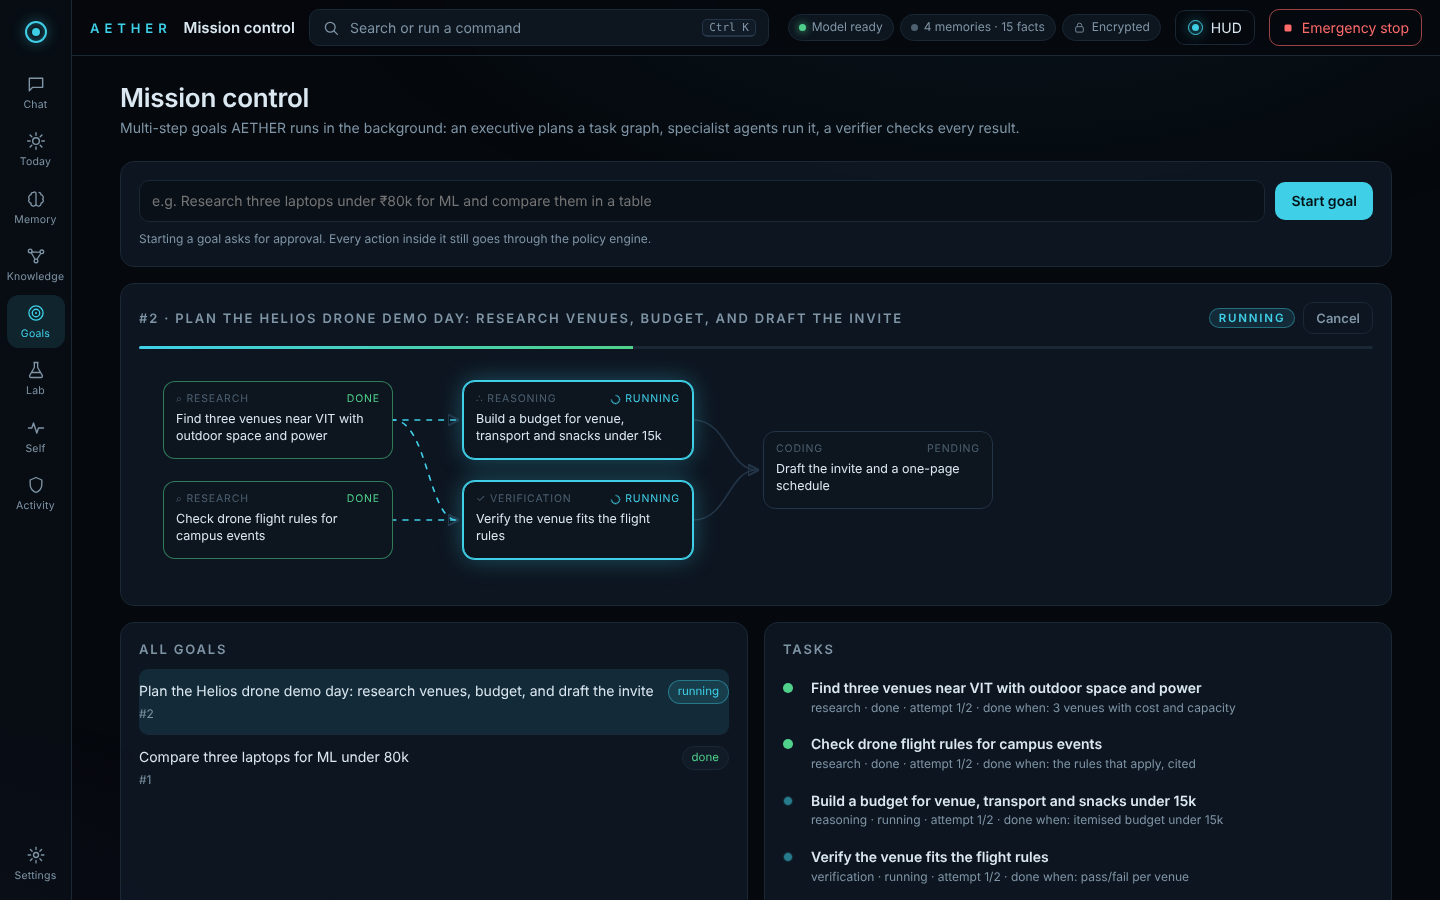
\includegraphics[width=\linewidth]{../screenshots/mission.png}
  \caption{Mission control for a goal mid-flight: two research tasks done, reasoning and verification running, the final task waiting on both.}
  \label{fig:mission}
\end{figure}

\subsection{HUD voice mode}
A full-screen voice interface (\code{Ctrl+Shift+H}) where the user holds Space to talk. The orb is drawn from real audio through WebAudio analysers: the microphone spectrum while listening and AETHER's synthesised voice while speaking. The current pipeline stage and a transcript are shown underneath.

\begin{figure}[h]
  \centering
  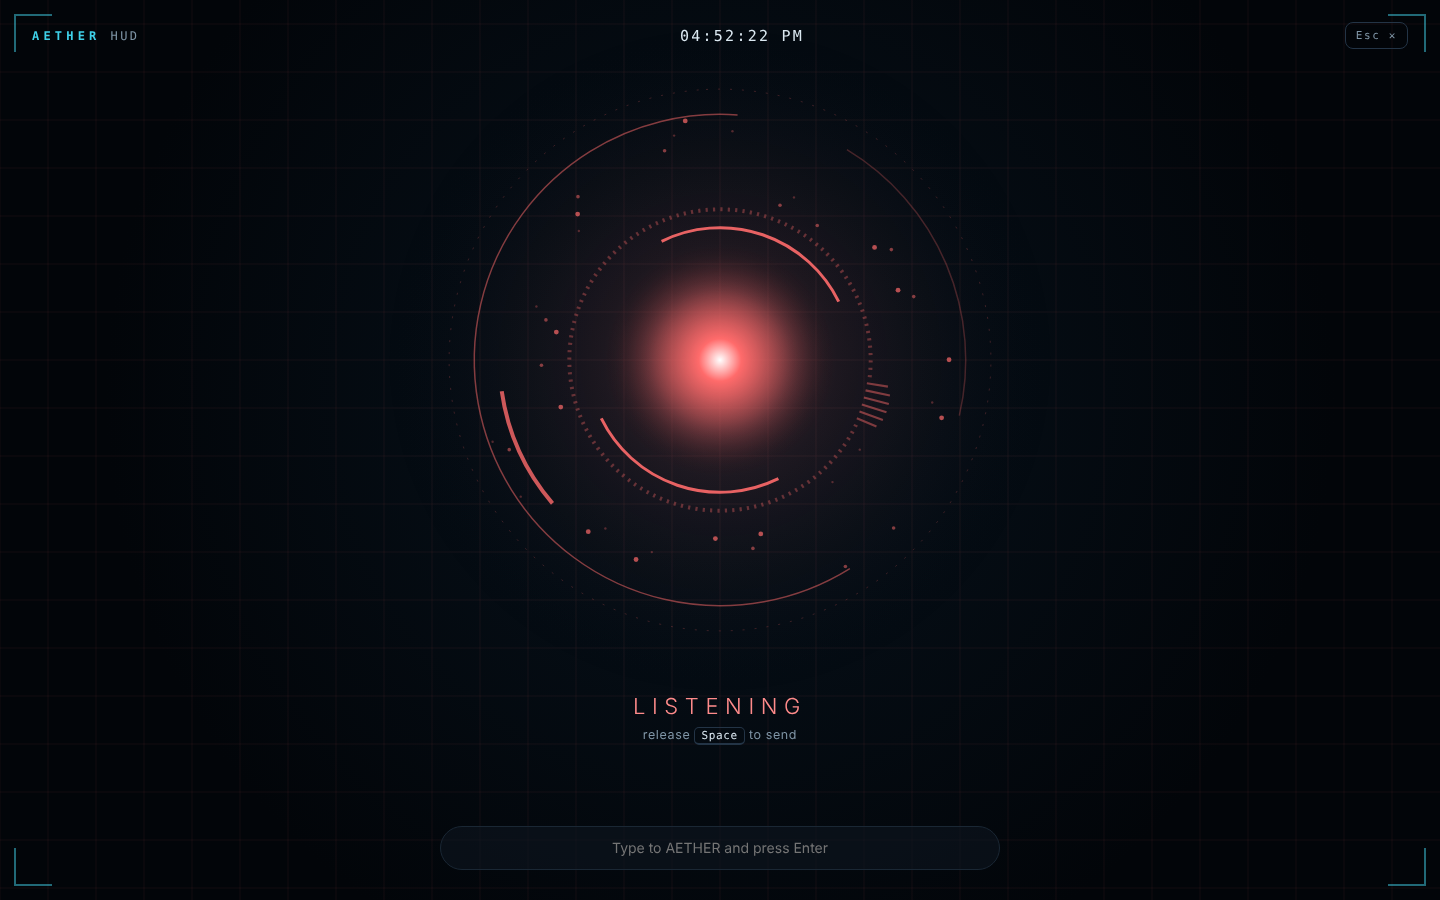
\includegraphics[width=0.49\linewidth]{../screenshots/hud-listen.png}\hfill
  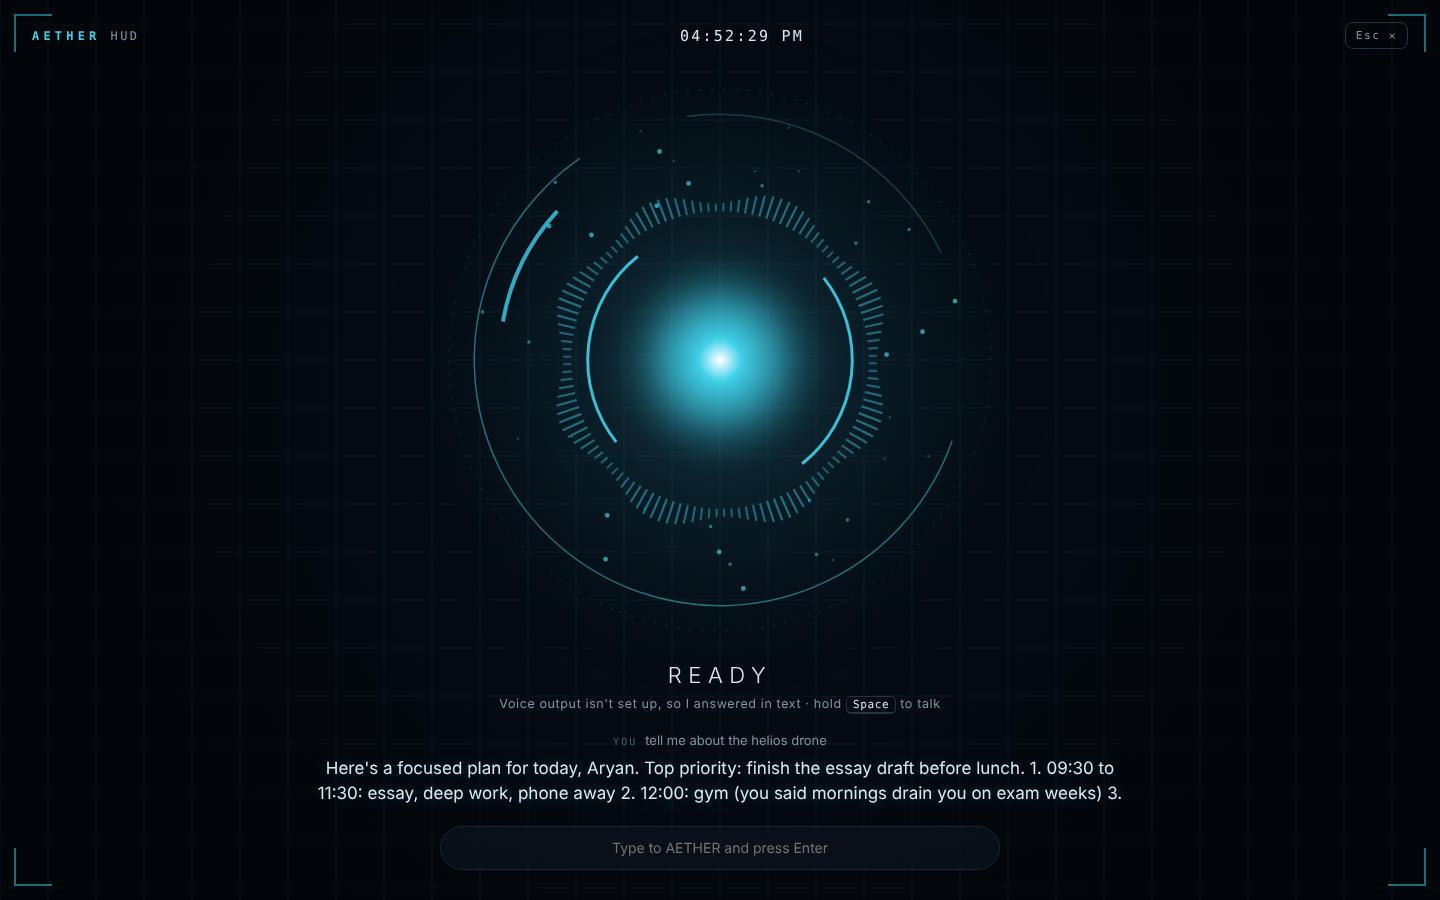
\includegraphics[width=0.49\linewidth]{../screenshots/hud-answer.png}
  \caption{HUD mode while listening (left) and after answering (right).}
\end{figure}

%=====================================================================
\section{Testing and evaluation}
\begin{itemize}
  \item \textbf{Unit and integration tests.} 122 tests (105 test functions, some parametrised) run in about 15 seconds with no model weights. A scripted language-model double, used only in tests, exercises every stage, the web API, streaming, traces, counterfactuals, time travel, security and the optimisers.
  \item \textbf{End-to-end scenarios.} \code{aether-eval} runs ten scenarios against the real model, judged by code: no retrieval for small talk, fact learning and contradictions, preference enforcement, crisis resources, listen-or-solve, cited document answers, injection resistance, topic switching, approval for deletes and the schedule optimiser.
  \item \textbf{Performance.} \code{scripts/bench.py} measures speed against the performance budget.
  \item \textbf{Browser checks.} Every view of the web app was driven in headless Chromium against the real server, including a simulated microphone for the HUD, and checked for console errors.
\end{itemize}

\subsection*{Known limits}
\begin{itemize}
  \item The system has been built and tested with a scripted model double. It has not yet run against real GGUF weights, a GPU, a microphone or Windows APIs; \code{aether-eval} and the benchmark are the first real check.
  \item Small local models follow instructions less reliably than large hosted models. The symbolic layer catches much of that, but answer quality still depends on the chosen model.
  \item The Tauri shell and the Inno Setup installer have not been compiled yet.
  \item The injection scanner is a tripwire; the policy engine and taint mode are the real guarantee.
\end{itemize}

%=====================================================================
\section{Development history}
\begin{center}
\small
\begin{tabularx}{\linewidth}{@{}r l X@{}}
\toprule
\# & Phase & What landed \\
\midrule
1 & Foundation and cognitive core & Chat, IR, knowledge graph, rules, memory, routing, preferences, wellness, policy, UI \\
2 & Memory depth & Vector index, memory extraction, topic summaries, reminders, decay \\
3 & Neuro-symbolic depth & Triples from documents, persisted user rules, first-order queries with proofs, CSP planner \\
4 & RAG and research & Folder watcher, reranker, cited research briefs, citation validation \\
5 & Agents and autonomy & Persistent task graph, executive, specialists and verifier, bounded retries, re-plan \\
6 & Computer control & App launch, sandboxed shell, trash and undo, OCR, UI automation \\
7 & Personalisation and desktop UI & Tauri shell, observation review, preference timeline \\
8 & Voice and multimodal & Wake word, STT and TTS with barge-in, image understanding \\
9 & Metaheuristics & NSGA-II, tabu search, differential evolution, optimisation lab, PSO self-tuning \\
10 & Metacognition & Turn metrics, feedback, self-review, approval-gated proposals \\
11 & Hardening & Encryption at rest, injection defence, proactive engine, evals, installer, performance budget \\
12 & Web app & Streaming chat with live pipeline, conversations, knowledge map, palette, voice, KV cache \\
13 & See inside it & Glass-box traces, counterfactuals, time travel, mission control, HUD \\
\bottomrule
\end{tabularx}
\end{center}
The code base is about 7\,000 lines of Python and 1\,800 lines of web front end, with no front-end build step and no external network dependencies beyond optional web search.

\section{Future work}
The next steps toward a true ``Jarvis'' are: always-on presence (tray app, global hotkey, wake word at start-up); screen awareness on request; voice routines such as ``focus mode'' built from policy-gated tools; a terse spoken persona; a local calendar read from \code{.ics} files; more proactive triggers (upcoming events, battery, deadlines); and lower voice latency through sentence-by-sentence speech and speculative decoding. All of these remain fully local.

\appendix
\section{Web API}
\begin{center}
\small
\begin{tabularx}{\linewidth}{@{}l X@{}}
\toprule
Endpoint & Purpose \\
\midrule
\code{POST /api/chat/stream} & Server-sent events: stages, tools, tokens, final answer with turn id \\
\code{GET /api/conversations} & List, open, rename, pin and delete saved conversations \\
\code{GET /api/search?q=} & Search memories, facts and conversations \\
\code{GET /api/graph?at=} & Knowledge graph, optionally as believed at time \code{at} \\
\code{GET /api/kg/history?entity=} & Belief history \\
\code{POST /api/whatif} & Counterfactual reasoning \\
\code{GET /api/traces/\{id\}} & Glass-box trace of one turn \\
\code{GET /api/goals/\{id\}} & Goal with its task graph \\
\code{POST /api/transcribe}, \code{/api/speak} & Local speech-to-text and text-to-speech \\
\code{POST /api/stop} & Emergency stop \\
\bottomrule
\end{tabularx}
\end{center}

\section{Repository layout}
\begin{lstlisting}
aether/
  core/            config, logging and audit, encryption at rest, settings overrides
  llm/             provider interface, llama.cpp and transformers providers, embeddings
  cognition/       IR, perception, router, context, orchestrator, trace recorder
  neurosymbolic/   knowledge graph, rules, CSP, policy, temporal, what-if, verifier
  memory/          layered store, vector index, extraction, reminders, lifecycle
  retrieval/       BM25, folder watcher, reranker, citations
  research/        cited research pipeline
  agents/          task graph, executive, specialists
  tools/           registry, filesystem, web, computer control
  personalization/ preferences, observations
  wellness/        companion and crisis handling
  optimization/    GA, SA, PSO, NSGA-II, tabu, DE, self-tuning
  metacognition/   metrics, feedback, self-review, proposals
  proactive/       triggers, quiet hours, notifications
  security/        prompt-injection scanner
  speech/          STT, TTS, VAD, wake word, voice loop
  perception/      local vision
  evals/           end-to-end scenarios
  interface/       CLI, FastAPI server, web app
desktop/  installer/  scripts/  tests/  docs/
\end{lstlisting}

\end{document}
